%\documentclass{winnower}
\documentclass[9pt]{article}
%\documentclass{article}
\usepackage{amssymb}
\usepackage{graphicx}
\graphicspath{{images/}}
\usepackage[margin=0.6in]{geometry}
\begin{document}

\title{A Comparative Study of Generative Adversarial Networks Towards Automatic Image Colorization}

\author{Cameron Fabbri}
\date{4/24/2017}

\maketitle

%-------------------------------------------------%
\section{Introduction}
%-------------------------------------------------%
Deep learning has recently shown impressive results towards various problems in multiple domains such as speech recognition,
image classification, image segmentation, and reinforcement learning. Until recently, much of the focus was towards
discriminative models, which aim to map a high-dimensional input, such as an image, to a class label. Deep generative models,
such as Deep Botlzmann Machines, Deep Belief Networks, and Autoencoders have not had the same level of success.
Generative Adversarial Networks (GANs) [1] are a class of generative models that have shown great success in generatig realistic
images. Despite their success, they are known to be very difficult to train, and are extremely sensitive to modifications.
For this reason it is not yet straightforward to directly apply them towards different problems or problems of a different domain.\newline

\noindent Since their introduction in 2014, there have been several large contributions made towards stabilizing and understanding
the training process of GANs. I will be focusing on implementing and comparing four different methods used for training GANs towards
the original problem of image generation. With these implemented, I apply their methods towards our goal to automatically
colorize grayscale images. The four different variants of GANs I will be focusing on are the original GAN formulation [1], Least Squares
GANs (LSGANs) [6], Energy-Based GANs (EBGANs) [4], and Wasserstein GAN (WGAN) [5]. The papers I will be discussing are [1,2,3,4,5,6], with additional
references to others not listed here. The original GANs paper [1] provides a novel method towards generating images with the use of an
adversarial loss, where both the generator and discriminator networks are multilayer perceptrons. Deep Convolutional GANs (DCGANs) [2]
bridge the gap between recent advances in deep learning and GANs by introducing deep convolutional generative adversarial networks. The architecture they contribute
is used in "pix2pix" [3], which approaches the problem of translating images from one domain to the other, in [4] which views the discriminator
as an energy function, in [5] which proposes to minimize an approximation of the Earth Mover distance, and in [6], which adopt the
least squares loss function in an attepmt to overcome the vanishing gradient problem commonly seen with GANs.

%-------------------------------------------------%
\section{Background and Related Work}
%-------------------------------------------------%

%-------------------------------------------------%
\subsection{Deep Learning}
%-------------------------------------------------%
Deep learning is a class of machine learning algorithms that use one or more \textit{hidden layers} between the input and output
to learn a hierarchy of concepts, often referred to as \textit{deep neural networks} (DNN).
In a feedforward network, or multilayer perceptron (MLP), each successive layer uses the output
from the previous layer as input, and uses an activation function, such as a logistic function, to obtain a new representation of the input. To
learn the set of weights and biases connecting successive layers, the error is propagated backwards through the network in order to optimize a
given objective function. This process is known as \textit{backpropagation}. Backpropagation is used in conjunction with an optimization method,
such as gradient descent, to efficiently compute the gradients by propagation from the output to input. This allows multi-layer networks to learn
a non-linear mapping from copious amounts of data. Because of the large amount of data needed to effectively train DNNs, \textit{stochastic gradient descent}
is often used via batches of data, which amounts to computing the gradient on a mini-batch of training samples. Recent advances in GPUs have
provided massive speedups in training due to their ability to parallelize the many operations in a DNN. \newline

%-------------------------------------------------%
\subsection{Convolutional Neural Networks}
%-------------------------------------------------%
\noindent The most common type of DNN for visual data is the Convolutional Neural Network (CNN), which is designed specifically for
multidimensional data such as images. CNNs incorporate three powerful techniques in order to achieve some degree of scale and shift invariance.
The first is the use of shared weights, which stems from the idea that a feature detector used in one part of an image is almost certainly useful in
other parts of the image. This also allows networks to reduce the number of parameters to avoid the curse of dimensionality. The second is the use of
local receptive fields. A kernel or filter is \textit{convolved} across the entire
image to produce a \textit{feature map}. Each pixel in the resulting feature map is the result of the kernel convolved with a small area in the input.
The use of local receptive fields allow earlier layers in the network to learn low-level features such as edges or corners, which can then be combined
in successive layers throughout the network to learn high-level features. The third technique is various forms of subsampling, such as the use of pooling
layers, which provide a form of nonlinear downsampling. Subsampling is performed to reduce the dimensionality of the internal representation. \newline

\noindent While the size of the output in a MLP is independent of the size of its input, in a CNN
the height and width of the resulting feature maps are dependent on the input as well as the size and stride of the kernel. The number of feature maps or \textit{depth} of the
resulting layer (which corresponds to the \textit{width} of the network as a whole) however, is arbitrary. Clearly, there are many different options to be chosen,
such as the size and stride of the kernel, and the number of feature maps to use. When designing a CNN, many rely on heuristics, as well as theorectical
design principles as shown in [17]. \newline%An example CNN architecture is shown in Figure 1. \newline

%-------------------------------------------------%
\subsection{Deep Generative Models}
%-------------------------------------------------%
\noindent Much focus has been put on CNNs as a discriminative model, learning a function to map some input data to some desired output label. In other words,
they learn the conditional distribution $P(y|x)$. The rest of this paper is focused on \textit{generative} models, which instead learn the joint
probability of the input data and labels. They attempt to model the data directly by learning $P(x,y)$. Autoencoders, Deep Boltzmann Machines, and
Deep Belief Nets are some examples of these class of models. Generative models are usually based on some generator network $G$, that takes as input
a random variable $z$ sampled from some distribution, e.g. $z \sim \mathcal{N}(0,1)$, and outputs a sample $x$. \newline

\noindent Generative models, as the name suggests, attempt to generate new data similar to existing data. Generative models have been shown to perform
well on many tasks such as inpainting, image denoising, and video generation. Autoencoders have been a popular form of generative model because of their
ability to approximate some distribution of observed data, such as imagery. A simple auto-encoder setup may be to learn an encoding $z$ over a set of images,
$\mathcal{X}$, with $z$ being of a much lower dimension than that of $X \in{\mathcal{X}}$. A training procedure for a setup such as this is as follows.
An image $X \in{\mathbb{R}^{m\times n}}$ is encoded through an encoder CNN to some latent variable $z \in{\mathbb{R}^{d}}$, which is then used as input to a
decoder CNN to produce $X' \in{\mathbb{R}^{m\times n}}$. A loss function, such as $L_2$, is then used to compare the two, and the error is propogated back through
the networks. To produce a new sample, a random variable $z' \sim \mathcal{N}$ can be used as input to the generator network in place of an encoded $z$. 
An open research problem is to determine an appropriate loss function. $L_2$ and $L_1$ often result in blurry images, and may not be a correct metric for
visual quality. A recent class of generative models proposes to instead use an \textit{adversarial} loss in place of existing loss functions in the form of
a network.

%\begin{figure}[!htb]
%   \begin{center}$
%      \begin{array}{cccc}
%         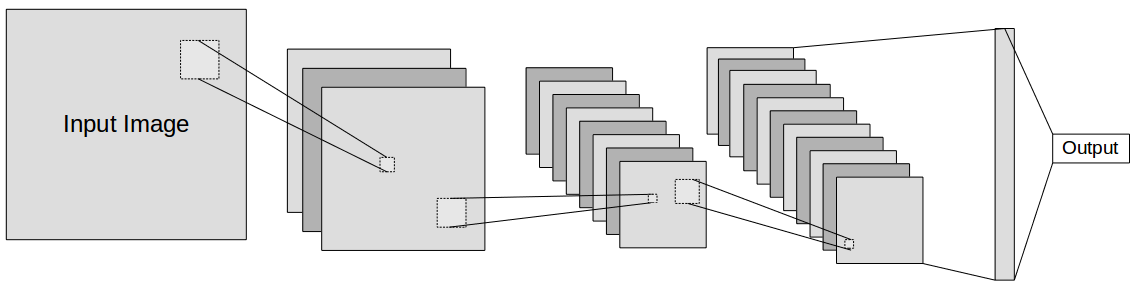
\includegraphics[width=3in]{cnn}
%      \end{array}$
%   \end{center}
%   \caption{\textit{An example of a Convolutional Neural Network}}
%\end{figure}


%-------------------------------------------------%
\section{Generative Adversarial Networks}
%-------------------------------------------------%
\noindent Generative Adversarial Networks (GANs) [1] are a recent class of generative models that are based on a game theory scenario in which a generator
network is competing against an adversary. The goal is to train a generator network to generate samples that are indistinguishable from the true data, $p_{data}$,
by mapping a random input variable $z \sim p_z$ to some some $\textbf{\textit{x}}$. This mapping can be represented as $G(z;\theta_g)$, where $G$ is a MLP with weights $\theta_g$, and $z$ is a random
variable sampled from some distribution, e.g. $z \sim \mathcal{N}(0,1)$. The discriminator, $D(\textbf{\textit{x}}; \theta_d)$ is represented by a second MLP with weights
$\theta_d$, and outputs a scalar representing the probability that a sample $\textbf{\textit{x}}$ came from $p_{data}$ rather than from $G$. The two networks are trained
simultaneously, with $D$ being trained to maximize the probability of correctly distinguishing whether or not a sample came from $p_{data}$ or from $G$, and $G$ being 
trained to fool $D$ by minimizing $log(1-D(G(z)))$. This can be represented by the following objective function:

\[\min\limits_{G}\max\limits_{D} \mathbb{E}_{x \sim p_{data(x)}} [logD(\textbf{\textit{x}})] + \mathbb{E}_{z \sim p_z(z)}[log(1 - D(G(z)))]\]

%\noindent GANs have been shown to optimize the Jensen-Shannon divergence (JSD)[1,7]. 
\noindent In practice however, $D$ will be able to discriminate between real and generated samples with
ease early in learning, due to the fact that generated images will clearly look very different than those from the training set upon initialization. As extensively shown in [7],
as $D$ gets better, the gradient begins to vanish. This means early in learning when $D$ is often perfect, it provides little or no gradients to $G$, so $G$ cannot improve.
To help avoid this issue, in practice $G$ is trained to maximize $logD(G(z))$, rather than minimize $log(1-D(G(z)))$, which is able to provide much stronger gradients. To validate the
results in [1], I implemented and trained MLP adversarial networks on the MNIST dataset [18] $^1$\footnote{Code for GAN and DCGAN results can be found
at https://github.com/cameronfabbri/DCGANs-Tensorflow}.\newline

\noindent Conditional GANs (cGANs) introduce a simple method to condition image generation on some extra information $y$ (e.g a class label). This is done by simply feeding
$y$ to the generator and discriminator networks along with $z$. The new objective function then becomes:

\[\min\limits_{G}\max\limits_{D} \mathbb{E}_{x \sim p_{data(x)}} [logD(\textbf{\textit{x}}|y)] + \mathbb{E}_{z \sim p_z(z)}[log(1 - D(G(z|y)))]\]

%\begin{figure}[!htb]
%   \begin{center}$
%      \begin{array}{cccc}
%         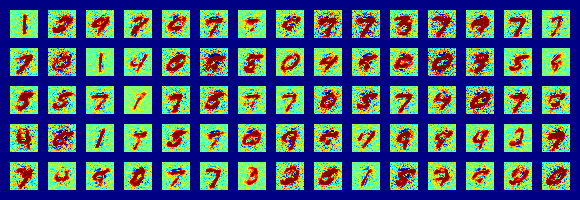
\includegraphics[width=3in]{gan_results}
%      \end{array}$
%   \end{center}
%   \caption{\textit{Results from training a GAN on MNIST after about 65 epochs.}}
%\end{figure}


%-------------------------------------------------%
\subsection{Deep Convolutional GANs}
%-------------------------------------------------%
I now turn towards Deep Convolutional GANs (DCGANs) [2], and discuss their success in bridging the gap between CNNs and GANs. Three important modifications are demonstrated throughout
their network architecture. The first is the replacement of downsampling layers such as max or average pooling with strided convolutions. While both perform downsampling, the
all convnet architecture allows the network to learn its own downsampling, as opposed to a harsh cut such as max pooling. The second modification is the elimination of fully
connected layers on top of convolutional layers, as often seen in models designed for classification. The final modification is the use of Batch Normalization [9], which normalizes
the input to each node to have zero mean and unit variance. This showed to help prevent the generator from collapsing to generate a single sample. Batch normalization is \textit{not}
applied to the generator output and the discriminator input, as they resulted in model instability. As opposed to the \textit{maxout} [10] activation used for the discriminator in
[1], DCGANs use a LeakyReLU activation for all layers. As for the generator, the ReLU [11] activation is used in all layers except the output layer, which uses $tanh$ to match
with the input range of $z$, $[-1,1]$. \newline

\begin{figure}[!htb]
   \begin{center}$
      \begin{array}{cccc}
         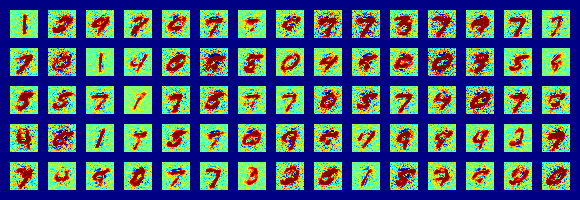
\includegraphics[width=3in]{gan_results} \hspace{10mm}
         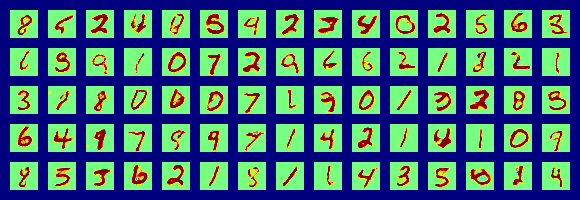
\includegraphics[width=3in]{dcgan_results}
      \end{array}$
   \end{center}
   \caption{Left: \textit{Results from training a GAN on MNIST.} Right: \textit{Results from training DCGANs on MNIST.}}
\end{figure}



\noindent The experiments provided show that their model acts as a very powerful generator for images in several domains. They evaluate their model on MNIST, the LSUN bedrooms dataset,
as well as human faces. To show the capabilities of their model beyond image generation, they successfully used it as a feature extractor for classification. Their DCGAN model
was trained on Imagenet-1k [12], and the features are then used for classification on CIFAR-10 images, achieving an accuracy of 82.8\%. A very impressive result is shown by modifying
the latent vector $z$ in order to manipulate the output of the generator. This is further explored in [13], which combines cGANs with an auto-encoder to control the attributes contained in generated
images in a more explicit manner. To compare with the results I obtained from [1], I implemented and trained a DCGAN on MNIST. Results can be seen compared to my implementation of GANs using a MLP in Figure 1,
and clearly contain much less noise$^1$.
    
%\begin{figure}[!htb]
%   \begin{center}$
%      \begin{array}{cccc}
%         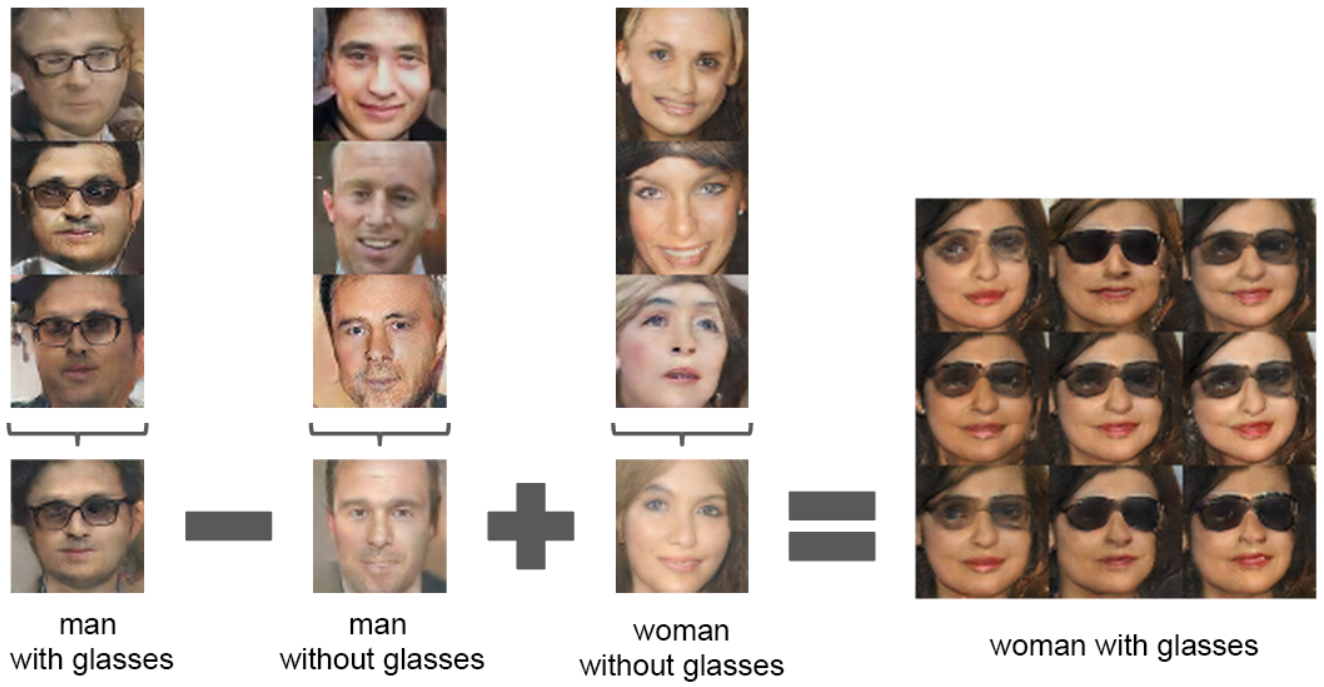
\includegraphics[width=3in]{faces}
%      \end{array}$
%   \end{center}
%   \caption{\textit{Modifications to the latent vectors $z$. For each column, the $z$ vector
%   used to generate the samples are averaged to produce the bottom image. Vector arithmetic
%   is then performed to produce a $z$ that is used to generate the center image on the right.
%   The extra images are the results of small modifications made to $z$ in the form of noise.
%   This image comes directly from} [2].}
%\end{figure}


%-------------------------------------------------%
\subsection{Least Squares GANs}
%-------------------------------------------------%
Least Squares GANs (LSGANs) attempt to overcome the problem of the vanishing gradient seen in the original GAN formulation by using the least squares loss function for the
discriminator. This is motivated by the idea that because [1] uses a cross entropy loss function for the discriminator, it is possible that generated samples on the correct side of the
decision boundary may still be far from the true data. The least squares loss is able to penalize samples that lie far from the decision boundary, and pull fake samples towards the
true data. The objective functions for $D$ and $G$ are defined as:

\[\min\limits_{D} \frac{1}{2} \mathbb{E}_{x \sim p_{data(x)}} [(D(\textbf{\textit{x}})-b)^2] + \frac{1}{2} \mathbb{E}_{z \sim p_z(z)}[(D(G(z)) - a)^2]\]
\[\min\limits_{G} \frac{1}{2} \mathbb{E}_{x \sim p_{data(x)}} [(D(G(\textbf{\textit{x}}))-c)^2] \]

\noindent where $a=0$ to denote the fake data, $b=1$ to denote the true data, and $c=1$ in order to try and fool $D$. The authors note that other values
may be used, such as setting $c=b$ in order to push $G$ to generate samples as real as possible, or by setting $b-c=1$ and $b-a=2$ to minimize the Pearson
$\mathcal{X}^2$ divergence between $p_{data}+p_g$ and $2p_g$, as opposed to minimizing the Jensen-Shannon divergence (JSD) as seen in the original GAN
formulation. In practice however, all show similar performance. \newline

\noindent Their experiments show sharp images generated at size $128\times128$, as opposed to the $64\times64$ images generated in [2]. Despite doubling
the resolution, the images are much clearer. Evaluations were done on multiple classes from the LSUN dataset. The architecture for both the discriminator
and generator are very similar to those used in DCGANs, with layers added to account for the increase in resolution. I implemented and trained LSGANs on the churches
class of LSUN \footnote{Code for LSGANs and more results on other LSUN classes can be found at https://github.com/cameronfabbri/LSGANs-Tensorflow}.
Results can be seen in Figure 2.
One important thing to note is the extreme diversity seen in the results, showing that LSGANs are able to avoid mode collapse for the generator.

\begin{figure}[!htb]
   \begin{center}$
      \begin{array}{cccc}
         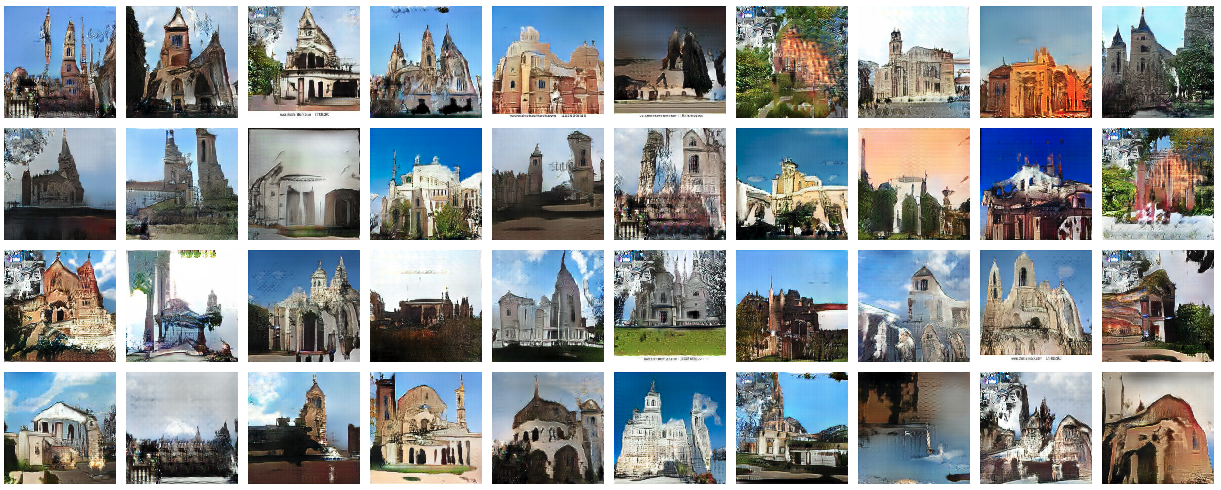
\includegraphics[width=3in]{least_squares_results2}
      \end{array}$
   \end{center}
   \caption{\textit{Results from training LSGANs on churches from the LSUN dataset. Note these are 128x128 images.}}
\end{figure}


%-------------------------------------------------%
\subsection{Energy-Based GANs}
%-------------------------------------------------%

Energy-Based GANs (EBGANs) [4] differ by treating the discriminator as an energy function that attributes low energies to the true samples and high energies
to generated samples. The generator is trained to generate samples with low energies. Attributing an energy to the discriminator allows for the possibility
of different loss functions in place of or combined with the usual cross entropy used in [1].  This paper chooses to use a margin loss, but point out that other
choices are available as shown in [14]. The loss for the generator $\mathcal{L}_G$ and discriminator $\mathcal{L}_D$ are formally defined as:

\[ \mathcal{L}_D(x,z) = D(x) + max(0, (m - D(G(z))) \]
\[ \mathcal{L}_G(z) = D(G(z)) \]

\noindent where $m$ is a positive margin. The authors claim that modeling the discriminator as an energy function offers higher stability when training
and leads to higher quality samples. The discriminator is structured as an auto-encoder with a mean squared error loss. The authors argue this for two
reasons. First, the reconstruction within the auto-encoder offers a more diverse set of targets for the discriminator rather than the binary outputs used
in [1]. Second, auto-encoders have the ability to learn an energy manifold \textit{without} supervision. For example, given only real images, a discriminator
modeled as an auto-encoder will be able to learn the data manifold on its own, which is in contrast to a discriminator trained for binary classification,
which doesn't make sense if given only one class. \newline

\noindent A common problem that often occurs during the training of GANs is the generator collapsing towards producing the same sample. To avoid this,
a pullaway term (PT) is introduced in order to decrease the samples visual similarity. The PT term aims to decrease the magnitude of the cosine similarity
between samples. The PT loss is used in the generator loss, but not the discriminator. Formally, with $S \in \mathbb{R}^{s\times N}$ representing a batch of images, it is defined as:

\[ PT(S) = \frac{1}{N(N-1)} \sum_i{\sum_{j\neq i}{(\frac{S^T_iS_j}{||S_i||||S_j||})^2}}\]

\noindent With this added PT loss, the loss for the generator becomes:

\[ \mathcal{L}_G(z) = D(G(z)) + \lambda PT \]

\noindent where $\lambda$ is a scaling term. In the paper, $\lambda$ was chose to be 0.1. Similar to DCGANs and LSGANs, experiments were done on the LSUN and CelebA dataset.
Models were trained with and with out the PT loss, denoting the model as EBGAN-PT when the PT term is added. I implemented and trained an EBGAN on the CelebA dataset.
Results can be seen in Figure 3, and visually match those presented in the paper\footnote{Code for EBGAN results can be found at: https://github.com/cameronfabbri/EBGAN-Tensorflow}.

\begin{figure}[!htb]
   \begin{center}$
      \begin{array}{cccc}
         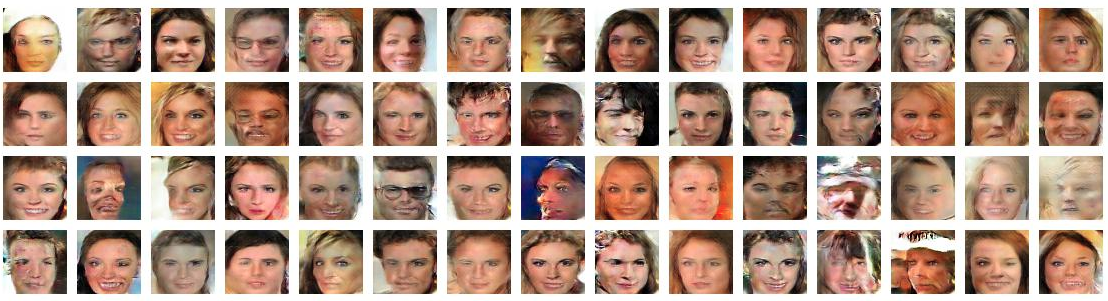
\includegraphics[width=4in]{ebgan0_results2}
      \end{array}$
   \end{center}
   \caption{\textit{Results from training EBGAN on faces from the CelebA dataset.}}
\end{figure}


%-------------------------------------------------%
\subsection{Wasserstein GANs}
%-------------------------------------------------%
Wasserstein GANs (WGAN) [5] explore several types of distance metrics between two distributions. In particular, they highlight the differences
between the JSD and the Earth Mover (EM) distance. In it's original formulation, GANs have been shown to optimize the JSD, defined as:

\[JSD(\mathbb{P}_r||\mathbb{P}_g) = \frac{1}{2} KL(\mathbb{P}_r || \mathbb{P}_A) + \frac{1}{2}KL(\mathbb{P}_g || \mathbb{P}_A)\]

\noindent where $\mathbb{P}_A = \frac{1}{2}(\mathbb{P}_r + \mathbb{P}_g)$, and $KL$ is the Kullback-Leibler divergence. As discussed thoroughly in [7] and shown through a simple example
in [5], this distance metric when used in sequences of probability distributions suffers from the vanishing gradient problem, where as the EM distance does not. The EM distance or
\textit{Wasserstein} is defined as:

\[ W(\mathbb{P}_r, \mathbb{P}_g) = inf_{\gamma \in \prod (\mathbb{P}_r, \mathbb{P}_g)} \mathbb{E}_{({x,y})\sim \gamma} [ || x - y || ] \]

\noindent where $\prod (\mathbb{P}_r, \mathbb{P}_g)$ denotes the set of joint distributions $\gamma (x,y)$ whose marginals are $\mathbb{P}_r$ and $\mathbb{P}_g$, respectively [5]. Because
the infimum is very troublesome, they instead propose to approximate $W$ given a set of $K$-Lipschitz functions $f$ by solving the following:

\[ \max\limits_{w \in W} \mathbb{E}_{x \sim \mathbb{P}_r}[f_w(x)] - \mathbb{E}_{z \sim p(z)}[f_w(G_{\theta}(z))]\]

\noindent Not surprisingly, such a function $f_w$ can be found by training a neural network. To ensure this function is $K$-Lipshitz, the weights are clamped to some range. In the paper, weights
are clamped to $[-0.1, 0.1]$, however I found a range of $[-0.05, 0.05]$ to produce better results.
Unlike in [1] where updates get consistently worse as the discriminator gets better, because the EM distance is continuous and differentiable, the WGAN discriminator (which is called the critic
because it is no longer a classifier) is trained to optimality. In their experiments, they performed one update on the generator for every five updates on the critic. This results in far better
gradients for the generator at the expense of very slow training. Furthermore, it was found that a very small learning rate must be used ($\alpha = 5e-5$) in order to avoid model divergence,
slowing training further. I implemented and trained a WGAN on the CelebA dataset, for which results can be seen in Figure 4 \footnote{Code for WGAN results can be found at:
https://github.com/cameronfabbri/Wasserstein-GAN-Tensorflow}.
Although the samples are visually similar to the EBGAN results, training took several days, as opposed to several hours for EBGAN. \newline

\begin{figure}[!htb]
   \begin{center}$
      \begin{array}{cccc}
         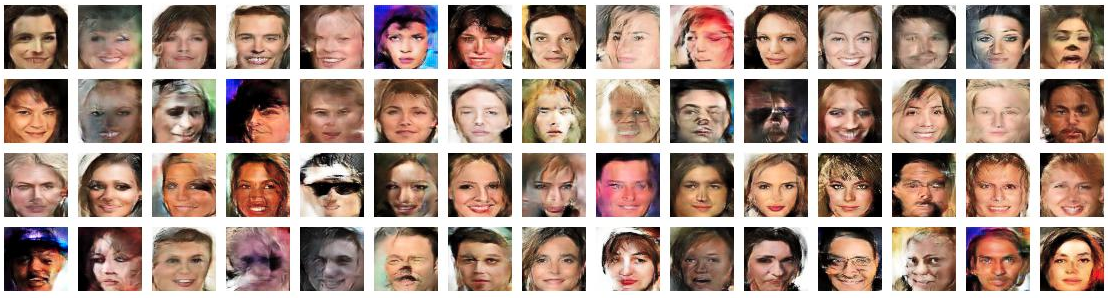
\includegraphics[width=4in]{wgan_results2}
      \end{array}$
   \end{center}
   \caption{\textit{Results from training WGAN on faces from the CelebA dataset.}}
\end{figure}

\noindent One very nice property of the WGAN that is not seen in the other GAN variants mentioned is a meaningful loss function that directly correlates with image quality. Figure 5 shows
the generator and discriminator losses for the DCGAN trained for generating the MNIST images in Figure 1 compared with the generator and critic losses for the WGAN trained for CelebaA results
in Figure 4. While visual quality improves in both models, only the WGAN losses appear to converge, while the DCGAN losses remain stable, making it impossible to gauge how well the model is performing.
Plotting the losses for LSGANs and EBGANs gives a similar result to that of DCGANs, providing little to no information on convergence $^{2,3}$.

\begin{figure}[!htb]
   \begin{center}$
      \begin{array}{cccc}
         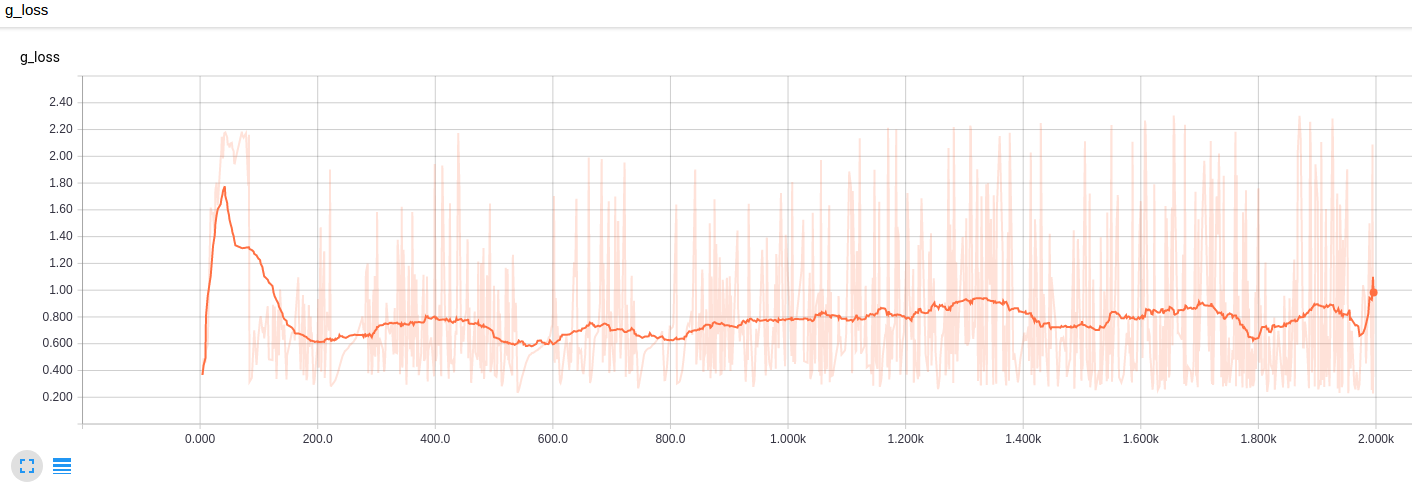
\includegraphics[width=2.7in]{dcgan_errG}
         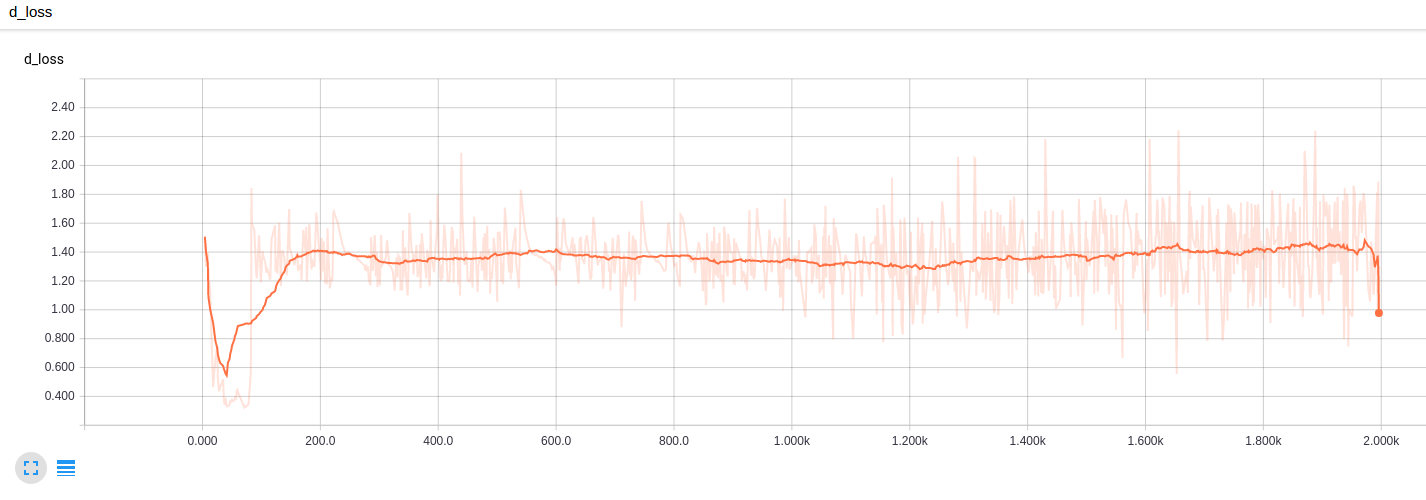
\includegraphics[width=2.7in]{dcgan_errD} \\
         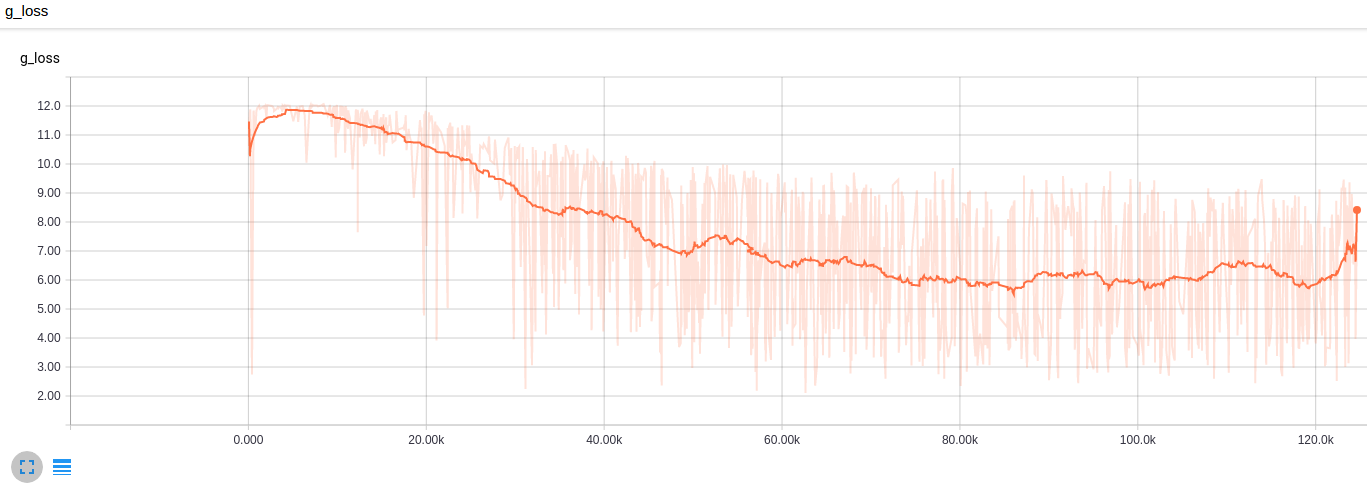
\includegraphics[width=2.7in]{wgan_errG}
         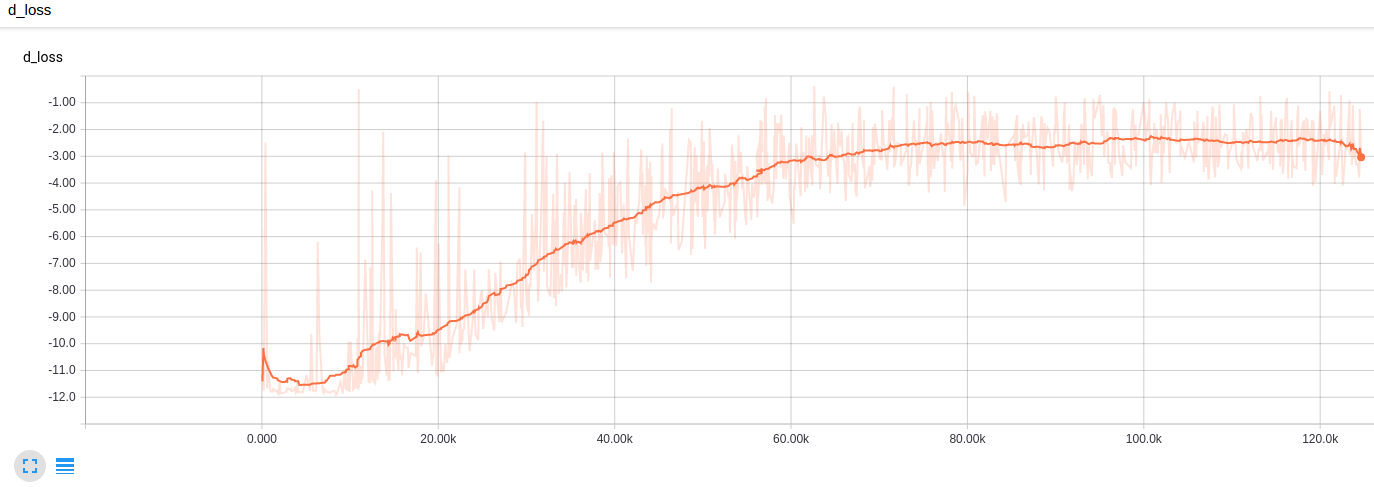
\includegraphics[width=2.7in]{wgan_errD}
      \end{array}$
   \end{center}
   \caption{Top Row: \textit{Generator and Discriminator losses, respectively for DCGANs.} Bottom Row: \textit{Generator and Discriminator losses, respectively for WGAN.
   While visual quality is increasing in both models, the WGAN loss clearly shows convergence that correlates with visual quality, while the loss for DCGANs stays constant.
   }}%Graphs generated with Tensorboard} [16].}
\end{figure}

%-------------------------------------------------%
\section{Colorization Approach}
%-------------------------------------------------%
I now show how adversarial networks can be used for generating a plausible color version of a grayscale image. The problem is set up as a cGAN, where the generator and discriminator
are both conditioned on the grayscale image. "Pix2pix" [3] presented a general approach towards translating an image from one domain to another. One such domain transformation was that of
grayscale to color. Their approach made use of combining an adversarial loss with $L_1$, which is a more traditional loss. This gives the model some sense of ground truth without it
being the only explicit form of loss. This combination turns out to be very helpful because in practice $L_1$ and $L_2$ produce blurry images. In theory, blurry
images should be rejected by the discriminator, thus pushing the generator to generate a sharp image while still being close to ground truth. \newline

\noindent Many deep learning architectures are designed around tasks that map a high dimensional input (such as an image) to a low dimensional output (such as a label). Early layers in
the network are able to learn low level features such as edges and corners, which are used in subsequent layers to learn higher level features. As a result, these low level features are
somewhat lost as you progress through the network, which for problems such as classification is okay, given the output of the network is ultimately a label. For tasks such as
image-to-image translation, where the network's output is visually very similar to the input, these low level features are important. For example, in the case of colorization, the
output color image has very similar edges and corners as the input grayscale image. It is for this reason that [3] chooses to use skip connections in their network, which concatenates the
activations from layer $i$ to layer $n-i$, where $n$ is the total number of layers. Their generator architecture is set up as an encoder-decoder, with the discriminator set up as a PatchGAN,
which instead of classifying an image as real or fake, classifies a $N \times N$ patch in the image. This allows for a texture style loss given by the discriminator, which when combined with
the $L_1$ loss that enforces correctness at low level frequencies, works very well. Their experiments were performed on a number of different styles of image-to-image translation, showing
the generalizability of their architecture. Some of these included map to aerial photo, grayscale to color, and day to night (all reversible). \newline

\noindent I adopted and implemented their model architecture for the task of colorizing grayscale images, and experimented with the several variations of GANs discussed earlier. Along with combining $L_1$, I also
experimented with $L_2$ as well. While the objective function for the discriminator/critic stayed the same as in the original papers, the objective function for the generator was as follows for the original GAN loss (LSGAN,
EBGAN, WGAN generator objective functions follow in a similar pattern) with $\lambda_1$, $\lambda_2$, and $\lambda_3$ being hyperparameters.

\[ \mathcal{L}_G = \lambda_1 [log(1-D(G(z))] + \lambda_2 L_1 + \lambda_3 L_2 \]

\noindent I used the $LAB$ colorspace in place of $RGB$, as the Euclidean distances between colors better model that of human vision. The input to the generator
is the lightness channel $L$,
and the output is a $(n \times m \times 2)$ matrix representing the $ab$ channels of the image. The lightness channel is then concatenated in order to form the final generated image. The discriminator is shown both
true images and generated images (separately). I experimented on the CelebA dataset, for which results can be seen in Figure 9\footnote{Code for colorization results can be found at:
https://github.com/cameronfabbri/Colorizing-Images-Using-Adversarial-Networks}. Most surprising was the EBGAN with $L_1$ being able to generate hardly any color output. 
WGAN did not finish training for 8 epochs due to its extensive training time compared to the other methods, but still produced reasonable results.
Although highly objective, I think that LSGANs performed the best, taking into account the end goal is not to recover true color, but a \textit{plausible} color. %My thoughts are that the fact that
The discriminator has a very difficult job due to the structural similarity between the real and generated images in comparison to the classical adversarial setup of testing the discriminator against images generated from
noise. For LSGANs, even though the discriminator may be fooled, the image may not be close to the true data distribution, which the loss function takes account for. \newline


\begin{figure}[!htb]
   \begin{center}$
      \begin{array}{cccc}
      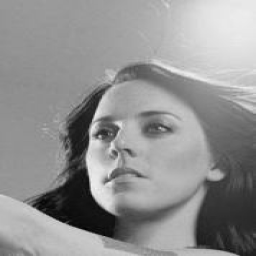
\includegraphics[width=0.70in]{1_gray} \hspace{1mm}
      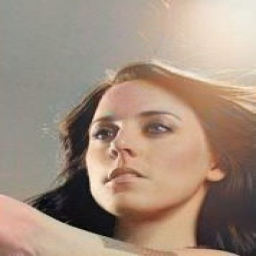
\includegraphics[width=0.70in]{1_gan_100_0_col}  \hspace{1mm}
      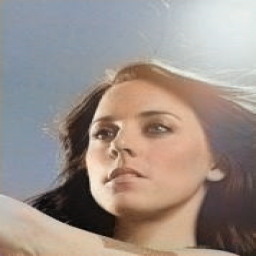
\includegraphics[width=0.70in]{1_gan_0_1_col} \hspace{1mm}
      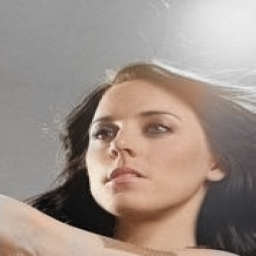
\includegraphics[width=0.70in]{1_lsgan_100_0_col} \hspace{1mm}
      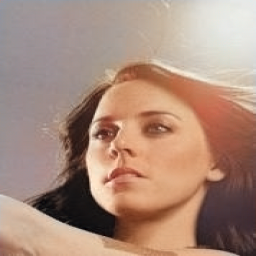
\includegraphics[width=0.70in]{1_lsgan_0_1_col} \hspace{1mm}
      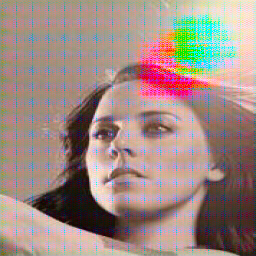
\includegraphics[width=0.70in]{1_ebgan_100_0_col} \hspace{1mm}
      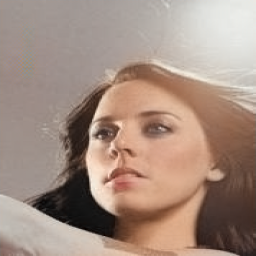
\includegraphics[width=0.70in]{1_ebgan_0_1_col} \hspace{1mm}
      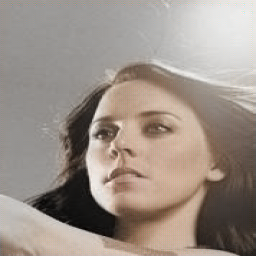
\includegraphics[width=0.70in]{1_wgan_100_0_col} \hspace{1mm}
      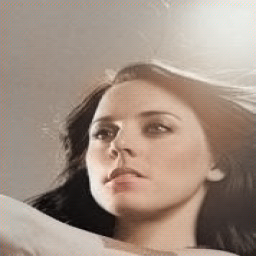
\includegraphics[width=0.70in]{1_wgan_0_1_col} \hspace{1mm}
      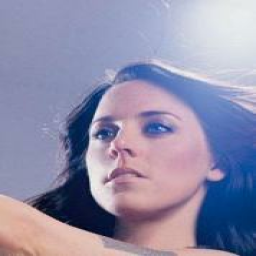
\includegraphics[width=0.70in]{1_true}
      \\
      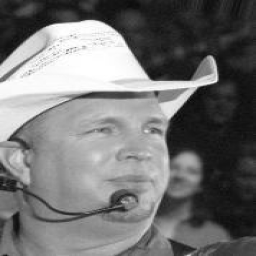
\includegraphics[width=0.70in]{2_gray} \hspace{1mm}
      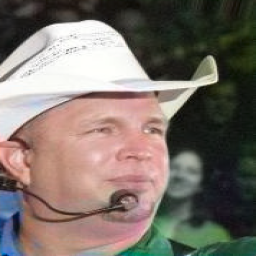
\includegraphics[width=0.70in]{2_gan_100_0_col} \hspace{1mm}
      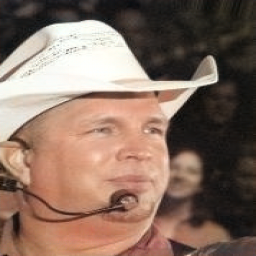
\includegraphics[width=0.70in]{2_gan_0_1_col} \hspace{1mm}
      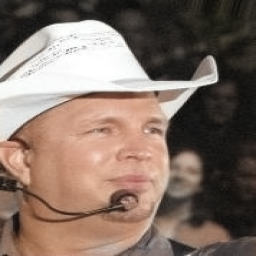
\includegraphics[width=0.70in]{2_lsgan_100_0_col} \hspace{1mm}
      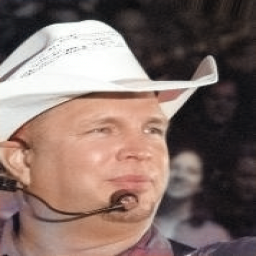
\includegraphics[width=0.70in]{2_lsgan_0_1_col} \hspace{1mm}
      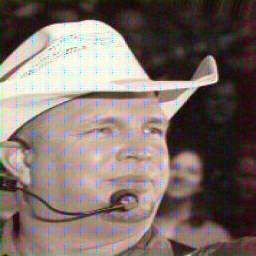
\includegraphics[width=0.70in]{2_ebgan_100_0_col} \hspace{1mm}
      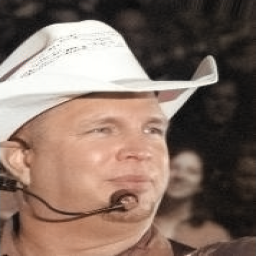
\includegraphics[width=0.70in]{2_ebgan_0_1_col} \hspace{1mm}
      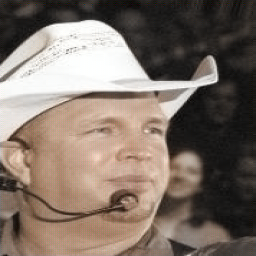
\includegraphics[width=0.70in]{2_wgan_100_0_col} \hspace{1mm}
      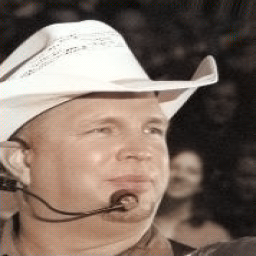
\includegraphics[width=0.70in]{2_wgan_0_1_col} \hspace{1mm}
      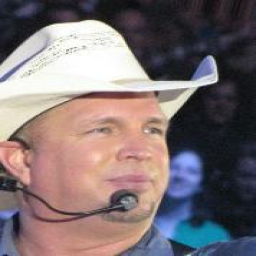
\includegraphics[width=0.70in]{2_true}
      \\
      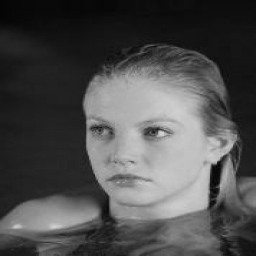
\includegraphics[width=0.70in]{3_gray} \hspace{1mm}
      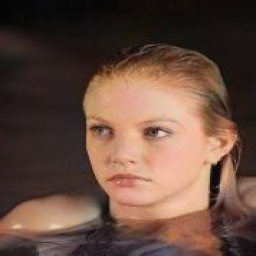
\includegraphics[width=0.70in]{3_gan_100_0_col} \hspace{1mm}
      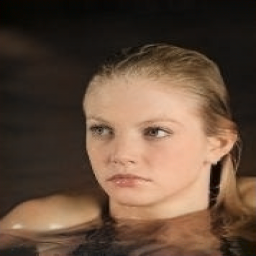
\includegraphics[width=0.70in]{3_gan_0_1_col} \hspace{1mm}
      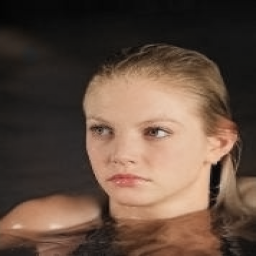
\includegraphics[width=0.70in]{3_lsgan_100_0_col} \hspace{1mm}
      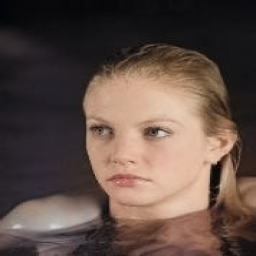
\includegraphics[width=0.70in]{3_lsgan_0_1_col} \hspace{1mm}
      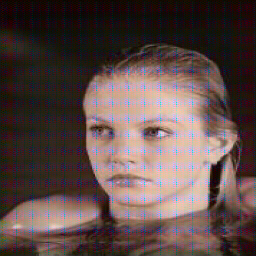
\includegraphics[width=0.70in]{3_ebgan_100_0_col} \hspace{1mm}
      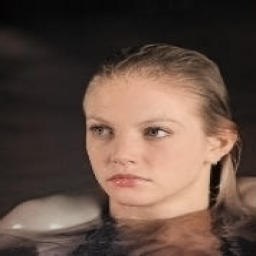
\includegraphics[width=0.70in]{3_ebgan_0_1_col} \hspace{1mm}
      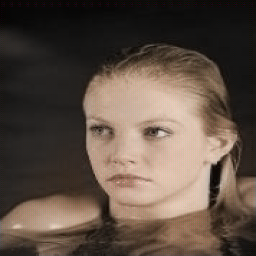
\includegraphics[width=0.70in]{3_wgan_100_0_col} \hspace{1mm}
      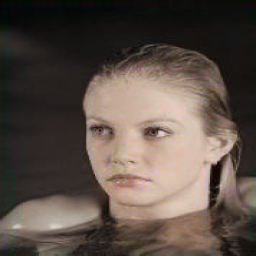
\includegraphics[width=0.70in]{3_wgan_0_1_col} \hspace{1mm}
      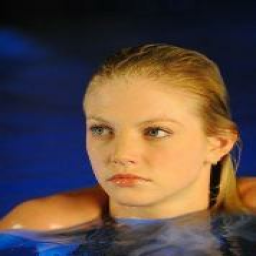
\includegraphics[width=0.70in]{3_true}
      \\
      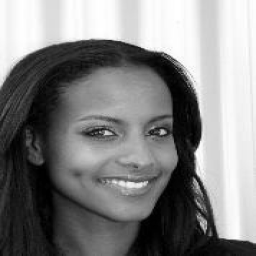
\includegraphics[width=0.70in]{4_gray} \hspace{1mm}
      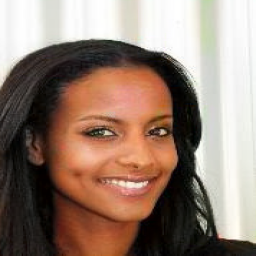
\includegraphics[width=0.70in]{4_gan_100_0_col} \hspace{1mm}
      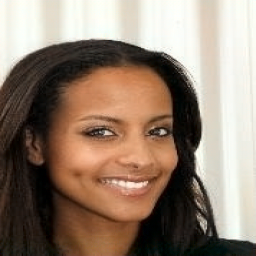
\includegraphics[width=0.70in]{4_gan_0_1_col} \hspace{1mm}
      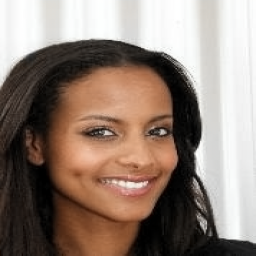
\includegraphics[width=0.70in]{4_lsgan_100_0_col} \hspace{1mm}
      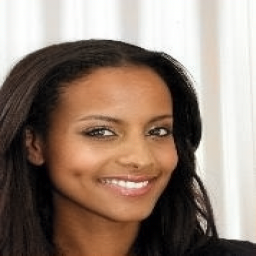
\includegraphics[width=0.70in]{4_lsgan_0_1_col} \hspace{1mm}
      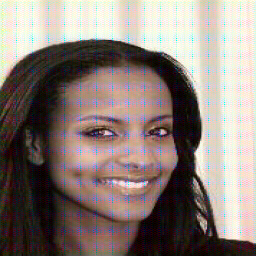
\includegraphics[width=0.70in]{4_ebgan_100_0_col} \hspace{1mm}
      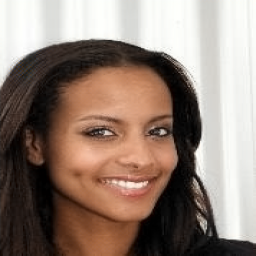
\includegraphics[width=0.70in]{4_ebgan_0_1_col} \hspace{1mm}
      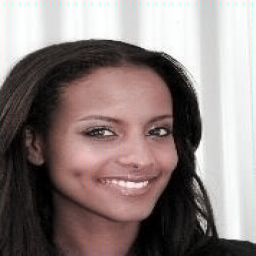
\includegraphics[width=0.70in]{4_wgan_100_0_col} \hspace{1mm}
      \includegraphics[width=0.70in]{4_wgan_0_1_col} \hspace{1mm}
      \includegraphics[width=0.70in]{4_true}
      \end{array}$
   \end{center}
   \caption{\textit{Variations from different models. $L_1$ and $L_2$ here refer to their respective $\lambda$ values in the objective function. From left to right: Input Image, GAN $L_1=100$ $L_2=0$, GAN $L_1=0$ $L_2=1$, 
   LSGAN $L_1=100$ $L_2=0$, LSGAN $L_1=0$ $L_2=1$,  EBGAN $L_1=100$ $L_2=0$,
      EBGAN $L_1=0$ $L_2=1$, WGAN $L_1=100$ $L_2=0$, WGAN $L_1=0$ $L_2=1$, True Image.}}
\end{figure}

\noindent It is important to note that because these are not "true" black and white images, what is being learned is the mapping from the function used to convert these images to grayscale back to color. To
compare, I also tested on true black and white images of John F. Kennedy and Muhammad Ali, seen in Figure 10. Note these images not only weren't trained on, but are completely outside of our dataset.

\begin{figure}[!htb]
   \begin{center}$
      \begin{array}{cccc}
         \includegraphics[width=0.75in]{gray_jfk} \hspace{1mm}
         \includegraphics[width=0.75in]{col_jfk_gan_0_1_1} \hspace{1mm}
         \includegraphics[width=0.75in]{col_jfk_gan_100_0_1} \hspace{1mm}
         \includegraphics[width=0.75in]{col_jfk_ls_100_0_1} \hspace{1mm}
         \includegraphics[width=0.75in]{col_jfk_ls_0_1_1} \hspace{1mm}
         \includegraphics[width=0.75in]{col_jfk_e_100_0_1} \hspace{1mm}
         \includegraphics[width=0.75in]{col_jfk_e_0_1_1} \hspace{1mm}
         \includegraphics[width=0.75in]{col_jfk_w_100_0_1} \hspace{1mm}
         \includegraphics[width=0.75in]{col_jfk_w_0_1_1} \\
         \includegraphics[width=0.75in]{gray_ali} \hspace{1mm}
         \includegraphics[width=0.75in]{ali_gan_0_1} \hspace{1mm}
         \includegraphics[width=0.75in]{ali_gan_100_0} \hspace{1mm}
         \includegraphics[width=0.75in]{ali_ls_100_0} \hspace{1mm}
         \includegraphics[width=0.75in]{ali_ls_0_1} \hspace{1mm}
         \includegraphics[width=0.75in]{ali_e_100_0} \hspace{1mm}
         \includegraphics[width=0.75in]{ali_e_0_1} \hspace{1mm}
         \includegraphics[width=0.75in]{ali_w_100_0} \hspace{1mm}
         \includegraphics[width=0.75in]{ali_w_0_1}

      \end{array}$
   \end{center}
   \caption{\textit{Colorizing true black and white photos. From left to right: Input Image, GAN $L_1=100$ $L_2=0$, GAN $L_1=0$ $L_2=1$,  LSGAN $L_1=100$ $L_2=0$, LSGAN $L_1=0$ $L_2=1$,  EBGAN $L_1=100$ $L_2=0$,
      EBGAN $L_1=0$ $L_2=1$, WGAN $L_1=100$ $L_2=0$, WGAN $L_1=0$ $L_2=1$. Note no true color images are available for these photos.}}
\end{figure}


\section{Conclusion and Future Work}
I explored various approaches towards training adversarial networks for image generation, and after verifying their results, applied their methods towards the ill-posed problem of automatically colorizing
a grayscale image. The combination of fine hyperparameter tuning and long turnaround time for results poses an inherent challenge. The training of GANs is highly unstable, and even the smallest of
changes may lead to inadequate results. %For example, a typo while training DCGANs that set the learning rate to $\alpha = 0.0001$ instead of $\alpha = 0.0002$ caused the output from the generator to lack
%any structure similar to MNIST.
Future work involves exploring these variations, as well as tackling the multiclass colorization problem.


\pagebreak

\section{References}
\bibliographystyle{abbrvnat}
\noindent [1] Goodfellow, Ian, Yoshua Bengio, and Aaron Courville. Deep learning. MIT Press, 2016. \newline
\noindent [2] Radford, Alec, Luke Metz, and Soumith Chintala. "Unsupervised Representation Learning with Deep Convolutional Generative Adversarial Networks." ICLR (2016): https://arxiv.org/abs/1511.06434. \newline
\noindent [3] Isola, Phillip, Zhoe, Efros. "Image-to-image translation with conditional adversarial networks." arXiv preprint arXiv:1611.07004 (2016). \newline
\noindent [4] Zhao, Junbo, Michael Mathieu, and Yann LeCun. "Energy-based generative adversarial network." arXiv preprint arXiv:1609.03126 (2016). \newline
\noindent [5] Arjovsky, Martin, Soumith Chintala, and Léon Bottou. "Wasserstein gan." arXiv preprint arXiv:1701.07875 (2017). \newline
\noindent [6] Mao, Xudong, et al. "Least squares generative adversarial networks." arXiv preprint ArXiv:1611.04076 (2016). \newline
\noindent [7] Arjovsky, Martin, and Léon Bottou. "Towards principled methods for training generative adversarial networks." NIPS 2016 Workshop on Adversarial Training. In review for ICLR. Vol. 2016. 2017. \newline
\noindent [8] Graves, Alex, and Navdeep Jaitly. "Towards End-To-End Speech Recognition with Recurrent Neural Networks." ICML. Vol. 14. 2014. \newline
\noindent [9] Ioffe, Sergey, and Christian Szegedy. "Batch normalization: Accelerating deep network training by reducing internal covariate shift." arXiv preprint arXiv:1502.03167 (2015). \newline
\noindent [10] Goodfellow, Ian J., et al. "Maxout Networks." ICML (3) 28 (2013): 1319-1327. \newline
\noindent [11] Nair, Vinod, and Geoffrey E. Hinton. "Rectified linear units improve restricted boltzmann machines." Proceedings of the 27th international conference on machine learning (ICML-10). 2010. \newline
\noindent [12] Deng, Jia, et al. "Imagenet: A large-scale hierarchical image database." Computer Vision and Pattern Recognition, 2009. CVPR 2009. IEEE Conference on. IEEE, 2009. \newline
\noindent [13] Perarnau, Guim, et al. "Invertible Conditional GANs for image editing." arXiv preprint arXiv:1611.06355 (2016). \newline
\noindent [14] LeCun, Yann, et al. "A tutorial on energy-based learning." Predicting structured data 1 (2006): 0 \newline
\noindent [15] Denton, Emily L., Soumith Chintala, and Rob Fergus. "Deep Generative Image Models using a Laplacian Pyramid of Adversarial Networks." Advances in neural information processing systems. 2015. \newline
\noindent [16] Abadi, Martín, et al. "Tensorflow: Large-scale machine learning on heterogeneous distributed systems." arXiv preprint arXiv:1603.04467 (2016). \newline
\noindent [17] Szegedy, Christian, et al. "Rethinking the inception architecture for computer vision." Proceedings of the IEEE Conference on Computer Vision and Pattern Recognition. 2016. \newline
\noindent [18] LeCun, Yann, Corinna Cortes, and Christopher JC Burges. "The MNIST database of handwritten digits." (1998). \newline
\noindent [19] Liu, Ziwei, et al. "Deep learning face attributes in the wild." Proceedings of the IEEE International Conference on Computer Vision. 2015. \newline

\bibliography{winnower_template}

\appendix

\end{document}
